%template for simulation report

\newpage

\section{Cassiopeia A}

\textbf{Object Description:}Ti-44 simulation

\textbf{Simulation Period:} February 2011 % month and year

\textbf{Science Team contract:}  Stephen Reynolds, Steven Boggs

\textbf{NuSIM configuration file:} CasA\_Ti.cfg

\textbf{Exposure time:}

\textbf{Input Source:} Chandra fits image in 4-6 kev and Fe line

\textbf{Tiling Method:} 5x5 rastering

\textbf{OA Database Version:} 008
% fill in version number e.g. 008

\textbf{Mast Bend Database:} SAA 90
% fill in SAA number

\textbf{Simulation notes:} The detector was moved over such that the optical axis was located at (-10,10) mm in detector module coordinates.
% did we learn anything, did we have to do something special?

\textbf{Status:} 
% are more simulations pending? is it missing something? 

\textbf{Location and name of simulation output:} resource/CasA/  in the nusim distribution.

\begin{figure}[ht]
  \begin{minipage}[c]{0.48\linewidth}
    \begin{center}
      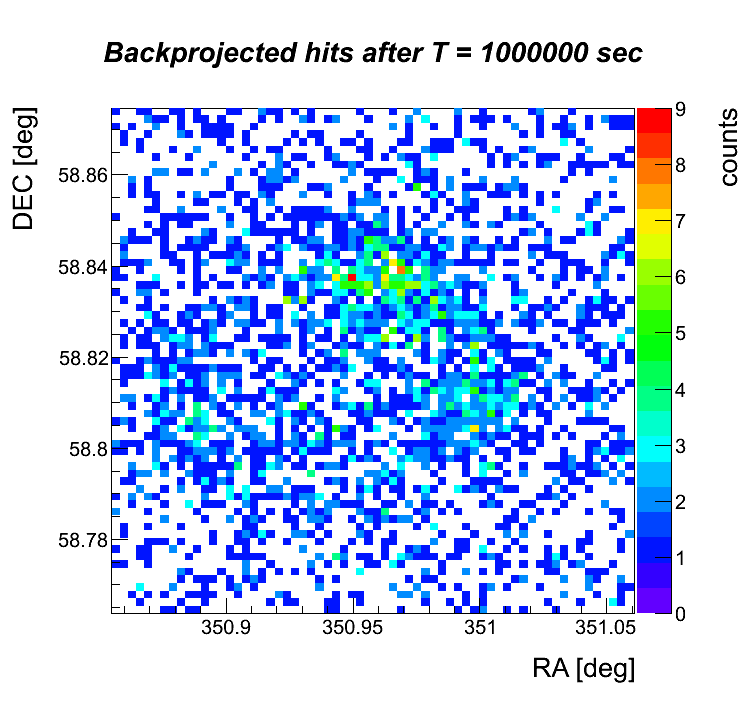
\includegraphics[scale=0.3]{CasA/CasA_It2b_B6_Smooth0.png}  
    \end{center}
  \end{minipage}
  \hspace{0.04\linewidth}
  \begin{minipage}[c]{0.48\linewidth}
    \begin{center}
      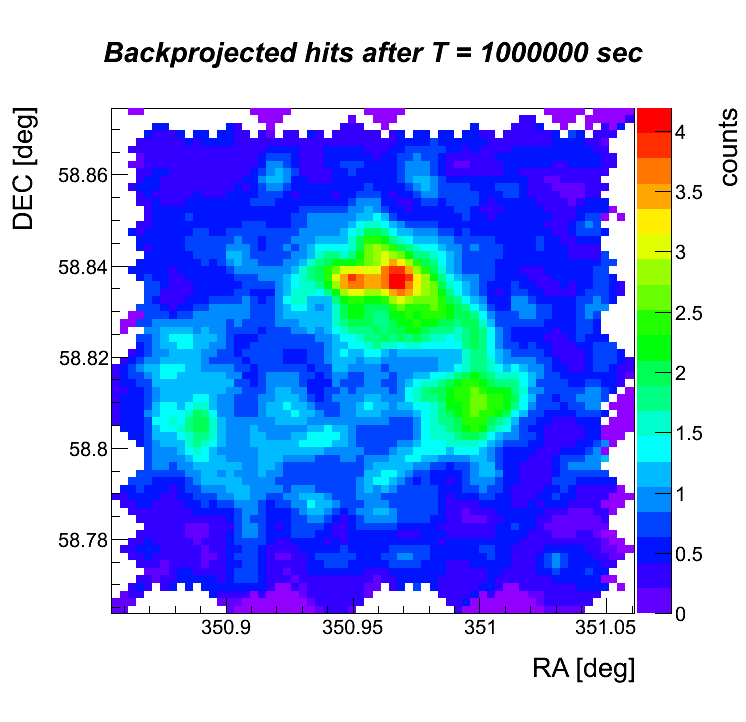
\includegraphics[scale=0.3]{CasA/CasA_It2b_B6_Smooth2.png}  
    \end{center}
  \end{minipage}
  \caption{Cassiopeia A, image is extracted in a 1.25 keV energy window around Ti-44 peak. Left: unsmoothed. Right: smoothed.}
\end{figure}

